\documentclass{kththesis}

\usepackage{blindtext} % This is just to get some nonsense text in this template, can be safely removed
\usepackage{multirow}
\usepackage{graphicx}

\usepackage{csquotes} % Recommended by biblatex
\usepackage{biblatex}
\addbibresource{references.bib} % The file containing our references, in BibTeX format


\title{Feature Selection Methods for Classification of Breast Cancer}
\alttitle{Attributurvalsmetoder för klassificering av bröstcancer}
\author{Niklas Lindqvist\newline Thony Price}
\email{nlinq@kth.se\newline thonyp@kth.se}
\supervisor{Pawel Herman}
\examiner{Orjan Ekeberg}
\programme{Degree Project in Computer Science}
\school{School of Computer Science and Communication}
\date{\today}


\begin{document}

% Frontmatter includes the titlepage, abstracts and table-of-contents
\frontmatter

\titlepage

\begin{abstract}
  >> This will be written later on...

  \blindtext
\end{abstract}


\begin{otherlanguage}{swedish}
  \begin{abstract}

    >> This will be written later on...

    Träutensilierna i ett tryckeri äro ingalunda en oviktig faktor,
    för trevnadens, ordningens och ekonomiens upprätthållande, och
    dock är det icke sällan som sorgliga erfarenheter göras på grund
    af det oförstånd med hvilket kaster, formbräden och regaler
    tillverkas och försäljas Kaster som äro dåligt hopkomna och af
    otillräckligt.
  \end{abstract}
\end{otherlanguage}


\tableofcontents


% Mainmatter is where the actual contents of the thesis goes
\mainmatter


\chapter{Introduction}

% We use the \emph{biblatex} package to handle our references.  We therefore use the command \texttt{parencite} to get a reference in parenthesis, like this \parencite{heisenberg2015}.  It is also possible to include the author as part of the sentence using \texttt{textcite}, like talking about the work of \textcite{einstein2016}.

Hospitals today are well equipped with data collection devices to do monitoring and data can be collected and shared in information systems. Collected data is a foundation for learning, both for medical personnel as well as for machines. As machine learning algorithms from the very beginning have been used to analyze medical data sets, machine learning is a well studied field within medical diagnosis \parencite{kononenko2001}. Computer aided diagnosis (CAD) makes use of machine learning techniques that learn a hypothesis, a statistical prediction about a patient's diagnose, from a large set of previously diagnosed examples in order to assist medical experts in making more accurate diagnostics more efficiently \parencite{li2007}.

Breast cancer is a disease of major concern and is the leading cause of cancer deaths among women \parencite{althuis2005}. At present there are no effective ways to prevent breast cancer. However, efficient diagnosis in an early stage can increase the chance of full recovery. This makes early detection and diagnosis an important issue and screening mammography is the primary imaging modality for early detection of breast cancer \parencite{tabar2001}.

Multiple studies of CAD on breast cancer have been conducted, primarily focusing on classifying mammography data as malignant or not, such those of \textcite{ramos2012} and \textcite{akay2009}. The act of feature selection, removing redundant or irrelevant features from a dataset, can provide classifiers to be faster, more cost-effective and accurate [8]. It is also explicitly mentioned as a topic in need of more research in a studies on breast cancer classification by \textcite{akin2011}.

\section{Research Question}

In our thesis we will study the impact of different feature selection methods on the classification rate of malignant breast cancer by different machine learning methods. We aim to answer the following:

\begin{itemize}
  \item Does the feature selection improve the accuracy of classification compared to using all features?
  \item In which machine learning methods does feature selection have the greatest impact?
  \item What features are most important for accurate classification of breast cancer?
\end{itemize}
   Our hypothesis is that overall the feature selection will improve the classification rate of all the machine learning methods used in this research scope. This hypothesis is based on previous research on this topic by \textcite{karabulut2012} where it was found that found classification improved by the use of filter methods for feature selection.
Our research differ the work presented in \parencite{karabulut2012} in the size of data sets data sets. In our project we will only use one data set and thus put more emphasis on breast cancer. The previous work did only investigate feature selection methods by filtering which we will extend with by implementing wrapper methods. Lasty, the research scope in this thesis includes a study of the effect of different feature selection methods on Support Vector Machines (SVM) which was not discussed by \parencite{karabulut2012}.

\section{Approach}

Trials will be conducted with feature selection Wrapper methods and feature selection Filter methods. The result of the feature selection methods will be used in a Decision Tree (DT), Support Vector Machine (SVM), Probabilistic Method (PM) and a Artificial Neural Network (ANN). See summary of implementations in \ref{table:methods}. The main reason for using these four methods \textbf{[insert better motivation here]} are that our knowledge in machine learning is limited and the four mentioned methods are the methods that we have previously studied. Also, the methods are well studied and there are several conducted studies which can be used for comparison.

\begin{table}[ht]
\begin{center}
\begin{tabular}{ |l|l| }
\hline
\multicolumn{2}{ |c| }{\textbf{Implementations}} \\
\hline
\multirow{4}{*}{Classifiers}
 & Decision Tree \\
 & Support Vector Machine \\
 & Probibalistic Method \\
 & Artificial Neural Network \\ \hline
\multirow{2}{*}{Feature Selection by Wrapping}
 & Recursive Feature Elimination (RFE) \\
 & Sequential Feature Selector (SFS) \\ \hline
\multirow{2}{*}{Feature Selection by Filter}
 & Chi-square \\
 & Entropy \\
\hline
\end{tabular}
\caption{All classifiers should be tested with each feature selection method.}
\label{table:methods}
\end{center}
\end{table}

A comparison of the classification rate on the machine learning methods without any feature selection and with feature selection will be conducted in order to establish the importance of feature selection in different machine learning approaches when classifying breast cancer. The evaluation criteria will primary be F1 score that conveys the balance between recall and precision of classification performance \parencite{muc1992}. Secondly, we will compare computational resources of the learning phase measured in time. The Breast Cancer Wisconsin (Diagnostic) Data Set \parencite{Dua:2017}, contains 569 instances with 32 attributes describing the features of breast cancer. Each instance is classified as benign (357) or malignant (212).

\section{Outline}

In the Background section earlier work on the topic will be more thouroughly presented on order to clearify how this thesis relates to the field. The following chapter, Methods will detail the methods used to achive the results that are presented in chapter 4.

\chapter{Background}

\section{Computer Aided Diagnostics}

Explain what it is

\section{Breast Cancer}

A study in Sweden by \textcite{tabar2001} found breast carcinoma mortality was reduced by 63\% after mammography was introduced. This clearly emphasize the benefits of screening which had resulted in a increased usage of the method to detect and diagnose breast cancer. The increasing demand for mammography image interpretation lead to a shortage of medical radiologist to perform this task and consequently non medical personnel supplement the mammography image interpretation (MII) \parencite{culpan2016}. As breast cancer continues to be the leading cause of cancer motality among women and more efficient diagnostics and pathology is high on demand the need of low-cost point-of-care is very much needed as stated by \textcite{martei2018}.

\section{Feature Selection}

The benefits of selecting a subset of all avaliable features are manyfold, among other it facilitates data visualization and data understanding, reduces the measurement and storage requirements and reduces training and utilization times. In cases with thousands of features it is essential to work with the data \parencite{guyon2003}.

\subsection{Filter methods}

Explain

\subsection{Wrapper methods}

Explain

\section{Related Work}

I guess we should focus here both on breast cancer diagnostics as well as progress in feature selection.

\chapter{Method}

\section{Data set}

The dataset used in this theises, Breast Cancer Wisconsin (Diagnostic) data set, was donated 1995 to UCI  Machine Learning Repository \parencite{Dua:2017} by one of its creators, Nick Street. It contains 569 instances with 32 attributes describing the features of breast cancer. Each instance is classified as benign (357) or malignant (212). The 32 attribute discribes ten real-value features which are:

\begin{itemize} \itemsep0pt \parskip0pt \parsep0pt
	\item \textbf{Radius:} Mean of distances from center to points on the perimeter.
	\item \textbf{Texture:} Standard deviation of gray-scale values.
	\item \textbf{Smoothness:} Local variation in radius lengths.
  \item \textbf{Compactness:} perimeter\textsuperscript{2} / area - 1.
  \item \textbf{Concavity:} Severity of concave portions of the contour.
  \item \textbf{Concave points:} Number of concave portions of the contour.
  \item \textbf{Fractal dimension:} Coastline approximation - 1.
  \item \textbf{Perimeter:} Local variation in radius lengths.
  \item \textbf{Area}
  \item \textbf{Symmetry}
\end{itemize}




\section{Implementation}

Detail on what algorithms we used

\section{Evaluation}

What methods are implemented to measure the results, are we using mean, standard deviation, f1 score, anova, how many times do we run etc...

\chapter{Results and analysis}

\section{Classification impovements}

Did classification improve, how, why

\begin{figure}[ht!]
  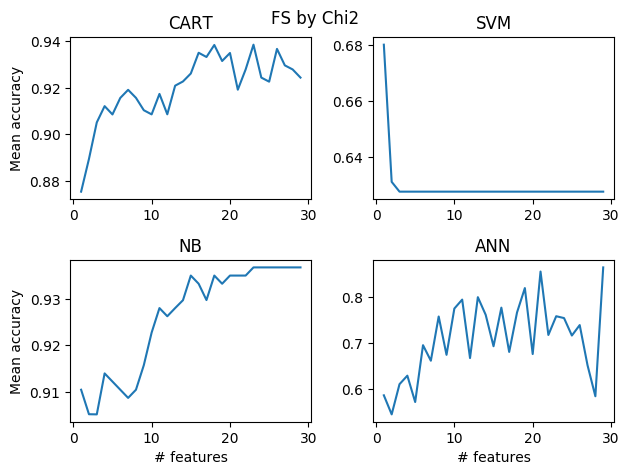
\includegraphics[width=\linewidth]{../plots/FS_by_Chi2.png}
  \caption{Performance by selecting features by Chi2}
  \label{fig:chi2}
\end{figure}

\begin{figure}[ht!]
  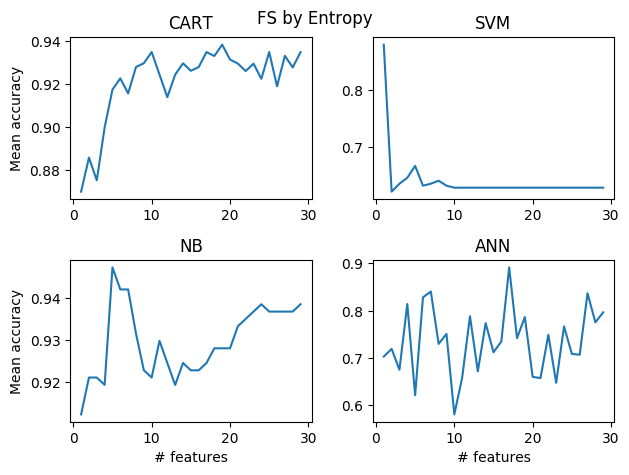
\includegraphics[width=\linewidth]{../plots/FS_by_Entropy.png}
  \caption{Performance by selecting features by Entropy}
  \label{fig:entropy}
\end{figure}

\begin{figure}[ht!]
  
\includegraphics[width=\linewidth]{../plots/RFS.png}
  \caption{Performance by selecting features by RFS}
  \label{fig:rfs}
\end{figure}

\section{Best features}

Could we tell which features contributes most to correct classification, how, why those

\section{Source of errors}

What can have caused faulty results, can our results be trusted?

\chapter{Discussion}

Let's discuss here

\chapter{Conclusion}

I guess this will be the last thing we write

\printbibliography[heading=bibintoc] % Print the bibliography (and make it appear in the table of contents)

\appendix

\chapter{Unnecessary Appended Material}

\end{document}
